% Rafael Sartori M. dos Santos, 186154
\documentclass[brazilian,a4paper]{article}

% Título
\title{MC832 -- Prova 2}
\author{Rafael Sartori M. Santos, 186154}
\date{12 de janeiro de 2021}

% Configuração do documento
%\setlength{\parskip}{3pt}
\usepackage[utf8]{inputenc} % tipo de documento UTF-8
%\usepackage{mathtools} % permitir expressões matemáticas
%\usepackage{breqn} % equações quebradas em várias linhas automaticamente
\usepackage{babel} % configuração da lingua portuguesa
\usepackage{caption} % para legenda de tabelas e figuras
\usepackage[
    pdfauthor={Rafael Sartori M. Santos},
    pdftitle={Prova 2 -- MC832},
    pdfproducer={LaTeX (texlive) com hyperref},
    hidelinks
]{hyperref} % para links externos (href)
\usepackage{cleveref} % para referenciar tabelas e figuras melhor
\usepackage{indentfirst} % indentação de todo primeiro parágrafo
\usepackage{graphicx} % para adicionar imagens
\graphicspath{{imgs-prova1/}} % atalho para o caminho das imagens
\usepackage{float} % para fixar posição de imagens
\usepackage{subcaption} % para imagens ficarem lado a lado
% Usamos geometry pois dá mais espaço que fullpage
%\usepackage{geometry} % alterar geometria do papel
%\geometry{a4paper,left=1.7cm,right=1.7cm,top=1cm,bottom=2.0cm} % menor margem
\usepackage{fullpage} % utilizamos uma versão com menos espaçamento nas bordas
\usepackage{verbatim} % pacote para incluir arquivos em verbatim
\usepackage{mdframed} % para enquadrar coisas
\usepackage[bitstream-charter]{mathdesign} % Mudamos a fonte para Charter BT
\usepackage[T1]{fontenc} % Mudamos a fonte para Charter BT

% Início do documento
\begin{document}

\maketitle

% https://classroom.google.com/u/1/c/MTQ4NTIwNTk0OTkx/a/MjQ5MDYyNzU5NDQ2/details

\section*{Exercício 1}

\textit{Network Address Translation} (NAT) é um recurso que surgiu para ``parametrizar'' redes, assim empresas e datacenteres não necessitariam atualizar os endereços de todos os servidores na mudança de provedores de internet, ao mover a rede ou ainda atualizar algum endereço público de um servidor específico. O recurso se popularizou para diminuir a quantidade de endereços IP devido a excassez causada pela inclusão digital e limites do IPv4.

Essa técnica pode ser empregada de vários jeitos em vários níveis. Pode ser utilizado para traduzir endereços, adicionar \textit{alias} para endereços públicos/privados e recursos mais avançados para servidores e \textit{firewalls}. É comum utilizarmos NAT em redes privadas como casas e pequenos comércios, em redes maiores como shopping centeres e empresas ou até internamente pelo provedor de internet para diminuir o uso de endereços IPv4. Neste caso, quanto maior o número de clientes, mais recursos (processamento e armazenamento) são necessários para fazer a tradução dos pacotes no envio e recebimento.

\begin{figure*}[h!]
    \centering
    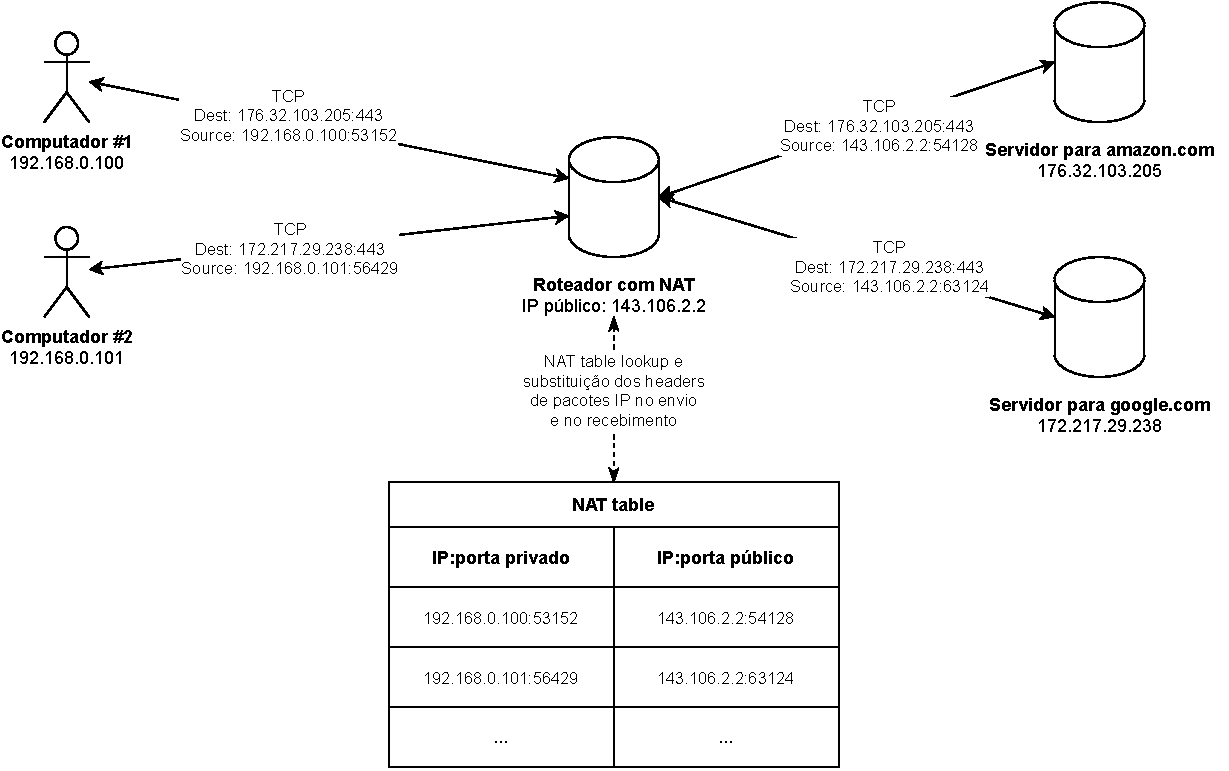
\includegraphics[width=0.9\textwidth]{prova2-nat.pdf}
    \caption{Ilustração do funcionamento de \textit{Network Address Translation} (NAT)}
    \label{fig-nat}
\end{figure*}

Como temos ilustrado na \cref{fig-nat}, a máquina que efetua a tradução (mais comumente um roteador) intercepta os pacotes enviados dos clientes, guarda em uma tabela as informações necessárias para que a tradução dos pacotes na volta seja possível e substitui os endereços. O pacote terá seu cabeçalho IP trocado por outro que utiliza o IP público e uma porta que será usada para traduzir os pacotes de volta (na volta, fazemos a troca contrária, removendo o IP público e retornando o IP privado com porta original).

Como o número de portas é limitado e várias aplicações utilizam várias conexões simultaneas, o endereço público pode ser esgotado, isto é, deixar de possuir portas livres para novas conexões, a depender da quantidade de conexões que os clientes utilizam e a quais servidores conectam. Para isso, o roteador pode ser melhorado (tanto em recursos computacionais quanto de software) para guardar mais informações na tabela, essencialmente repetindo portas para \textit{hosts} diferentes.

O NAT, portanto, é uma ideia bem ampla e dinâmica, o que possibilita a redução do uso de endereços IPv4 de forma muito eficiente e escalável, mas também possibilita recursos muito avançados em datacenteres e em redes complexas.


\section*{Exercício 2}

Figura explicando encaminhamento do roteador R1.


\section*{Exercício 3}

Explique funcionamento do CSMA-CA no Wi-Fi.

\end{document}
